\iffalse
\documentclass[journal,12pt,twocolumn]{IEEEtran}
\usepackage{romannum}
\usepackage{float}
\usepackage{setspace}
\usepackage{gensymb}
\singlespacing
\usepackage[cmex10]{amsmath}
\usepackage{amsthm}
\usepackage{mathrsfs}
\usepackage{txfonts}
\usepackage{stfloats}
\usepackage{bm}
\usepackage{cite}
\usepackage{cases}
\usepackage{subfig}
\usepackage{longtable}
\usepackage{multirow}
\usepackage{enumitem}
\usepackage{mathtools}
\usepackage{steinmetz}
\usepackage{tikz}
\usepackage{circuitikz}
\usepackage{verbatim}
\usepackage{tfrupee}
\usepackage[breaklinks=true]{hyperref}
\usepackage{tkz-euclide}
\usetikzlibrary{calc,math}
\usepackage{listings}
    \usepackage{color}                                            %%
    \usepackage{array}                                            %%
    \usepackage{longtable}                                        %%
    \usepackage{calc}                                             %%
    \usepackage{multirow}                                         %%
    \usepackage{hhline}                                           %%
    \usepackage{ifthen}                                           %%
  %optionally (for landscape tables embedded in another document): %%
    \usepackage{lscape}     
\usepackage{multicol}
\usepackage{chngcntr}
\DeclareMathOperator*{\Res}{Res}
\renewcommand\thesection{\arabic{section}}
\renewcommand\thesubsection{\thesection.\arabic{subsection}}
\renewcommand\thesubsubsection{\thesubsection.\arabic{subsubsection}}

\renewcommand\thesectiondis{\arabic{section}}
\renewcommand\thesubsectiondis{\thesectiondis.\arabic{subsection}}
\renewcommand\thesubsubsectiondis{\thesubsectiondis.\arabic{subsubsection}}

% correct bad hyphenation here
\hyphenation{op-tical net-works semi-conduc-tor}
\def\inputGnumericTable{}                                 %%

\lstset{
frame=single, 
breaklines=true,
columns=fullflexible
}

\begin{document}


\newtheorem{theorem}{Theorem}[section]
\newtheorem{problem}{Problem}
\newtheorem{proposition}{Proposition}[section]
\newtheorem{lemma}{Lemma}[section]
\newtheorem{corollary}[theorem]{Corollary}
\newtheorem{example}{Example}[section]
\newtheorem{definition}[problem]{Definition}
\newcommand{\BEQA}{\begin{eqnarray}}
\newcommand{\EEQA}{\end{eqnarray}}
\newcommand{\define}{\stackrel{\triangle}{=}}

\bibliographystyle{IEEEtran}
\providecommand{\mbf}{\mathbf}
\providecommand{\pr}[1]{\ensuremath{\Pr\left(#1\right)}}
\providecommand{\qfunc}[1]{\ensuremath{Q\left(#1\right)}}
\providecommand{\sbrak}[1]{\ensuremath{{}\left[#1\right]}}
\providecommand{\lsbrak}[1]{\ensuremath{{}\left[#1\right.}}
\providecommand{\rsbrak}[1]{\ensuremath{{}\left.#1\right]}}
\providecommand{\brak}[1]{\ensuremath{\left(#1\right)}}
\providecommand{\lbrak}[1]{\ensuremath{\left(#1\right.}}
\providecommand{\rbrak}[1]{\ensuremath{\left.#1\right)}}
\providecommand{\cbrak}[1]{\ensuremath{\left\{#1\right\}}}
\providecommand{\lcbrak}[1]{\ensuremath{\left\{#1\right.}}
\providecommand{\rcbrak}[1]{\ensuremath{\left.#1\right\}}}
\theoremstyle{remark}
\newtheorem{rem}{Remark}
\newcommand{\sgn}{\mathop{\mathrm{sgn}}}
\providecommand{\abs}[1]{\left\vert#1\right\vert}
\providecommand{\res}[1]{\Res\displaylimits_{#1}} 
\providecommand{\norm}[1]{\left\lVert#1\right\rVert}
\providecommand{\mtx}[1]{\mathbf{#1}}
\providecommand{\mean}[1]{E\left[ #1 \right]}
\providecommand{\fourier}{\overset{\mathcal{F}}{ \rightleftharpoons}}
\providecommand{\system}{\overset{\mathcal{H}}{ \longleftrightarrow}}
\newcommand{\solution}{\noindent \textbf{Solution: }}
\newcommand{\cosec}{\,\text{cosec}\,}
\providecommand{\dec}[2]{\ensuremath{\overset{#1}{\underset{#2}{\gtrless}}}}
\newcommand{\myvec}[1]{\ensuremath{\begin{pmatrix}#1\end{pmatrix}}}
\newcommand{\mydet}[1]{\ensuremath{\begin{vmatrix}#1\end{vmatrix}}}
\numberwithin{equation}{subsection}
\makeatletter
\@addtoreset{figure}{problem}
\makeatother

\let\StandardTheFigure\thefigure
\let\vec\mathbf
\renewcommand{\thefigure}{\theproblem}



\def\putbox#1#2#3{\makebox[0in][l]{\makebox[#1][l]{}\raisebox{\baselineskip}[0in][0in]{\raisebox{#2}[0in][0in]{#3}}}}
     \def\rightbox#1{\makebox[0in][r]{#1}}
     \def\centbox#1{\makebox[0in]{#1}}
     \def\topbox#1{\raisebox{-\baselineskip}[0in][0in]{#1}}
     \def\midbox#1{\raisebox{-0.5\baselineskip}[0in][0in]{#1}}

\vspace{3cm}


\title{Assignment 1}
\author{Jaswanth Chowdary Madala}





% make the title area
\maketitle

\newpage

%\tableofcontents

\bigskip

\renewcommand{\thefigure}{\theenumi}
\renewcommand{\thetable}{\theenumi}

\begin{enumerate}

\textbf{Solution:}
\fi
		The givne lines can be written  in vector form  as
\begin{align}
	\vec{x} &= \myvec{1\\1\\0} + \lambda_1\myvec{2\\-1\\1},
\vec{x} = \myvec{2\\1\\-1} + \lambda_2\myvec{3\\-5\\2}\\
\implies \vec{x_1} = \myvec{1\\1\\0},\, \vec{x_2} &= \myvec{2\\1\\-1}, \,\vec{m_1} = \myvec{2\\-1\\1}, \, \vec{m_2} = \myvec{3\\-5\\2}
\end{align}
%
We first check whether the given lines are skew. The lines 
\begin{align}
\vec{x} = \vec{x_1} + \lambda_1\vec{m_1},\, \vec{x} = \vec{x_2} + \lambda_2\vec{m_2} 
\label{eq:chapters/12/11/2/e11/1}
\end{align}
intersect if
\begin{align}
\vec{M}\bm{\lambda} &= \vec{x_2} - \vec{x_1}\\
\vec{M} &\triangleq \myvec{\vec{m_1} & \vec{m_2}} \\
\bm{\lambda} &\triangleq \myvec{\lambda_1\\-\lambda_2}\\
\end{align}
Here we have,
\begin{align}
\vec{M} &= \myvec{2&3\\-1&-5\\1&2},
\vec{x_2} - \vec{x_1} &= \myvec{1\\0\\-1}
\end{align}
We check whether the equation \eqref{eq:chapters/12/11/2/e11/2} has a solution
\begin{align}
\myvec{2&3\\-1&-5\\1&2}\bm{\lambda} = \myvec{1\\0\\-1}
\label{eq:chapters/12/11/2/e11/2}
\end{align}
The augmented matrix is given by,
\begin{align}
\myvec{2&3&\vrule&1\\-1&-5&\vrule&0\\1&2&\vrule&-1}
\xleftrightarrow[R_3 \leftarrow R_3 - \frac{1}{2}R_1]{R_2 \leftarrow R_2 + \frac{1}{2}R_1}
\myvec{2&3&\vrule&1\\&&\vrule\\0&-\frac{7}{2}&\vrule&\frac{1}{2}\\&&\vrule\\0&\frac{1}{2}&\vrule&-\frac{3}{2}}\\
\xleftrightarrow{R_3 \leftarrow R_3 + 7R_2}
\myvec{2&3&\vrule&1\\&&\vrule\\0&-\frac{7}{2}&\vrule&\frac{1}{2}\\&&\vrule\\0&0&\vrule&-10}
\end{align}
The rank of the matrix is 3. So the given lines are skew.
The closest points on two skew lines defined by \eqref{eq:chapters/12/11/2/e11/1} are given by 
\begin{align}
\vec{M}^\top \vec{M}\bm{\lambda} &= \vec{M}^\top\brak{\vec{x_2}-\vec{x_1}}\\
\implies \myvec{2&-1&1\\3&-5&2} \myvec{2&3\\-1&-5\\1&2}\bm{\lambda} &= \myvec{2&-1&1\\3&-5&2} \myvec{1\\0\\-1}\\
\implies \myvec{6&13\\13&38}\bm{\lambda} &= \myvec{1\\1}
\label{eq:chapters/12/11/2/e11/3}
\end{align}
The augmented matrix of the above equation \eqref{eq:chapters/12/11/2/e11/3} is given by,
\begin{align}
\myvec{6&13&\vrule&1\\13&38&\vrule&1}
\xleftrightarrow{R_2 \leftarrow R_2 - \frac{13}{6}R_1}
\myvec{6&13&\vrule&1 \\&&\vrule\\ 0&\frac{59}{6}&\vrule&-\frac{7}{6}}\\
\xleftrightarrow{R_1 \leftarrow R_1 - \frac{78}{59}R_2}
\myvec{6&0&\vrule&\frac{150}{59} \\&&\vrule\\ 0&\frac{59}{6}&\vrule&-\frac{7}{6}}
\end{align}
So, we get
\begin{align}
\myvec{\lambda_1\\-\lambda_2} &= \myvec{\frac{25}{59}\\\\-\frac{7}{59}}
\end{align}
The closest points $\vec{A}$ on line $l_1$ and $\vec{B}$ on line $l_2$ are given by,
\begin{align}
\vec{A} &= \vec{x_1} + \lambda_1\vec{m_1}
= \frac{1}{59}\myvec{109\\34\\25}\\
\vec{B} &= \vec{x_2} + \lambda_2\vec{m_2}
= \frac{1}{59}\myvec{139\\24\\-45}
\end{align}
The minimum distance between the lines is given by,
\begin{align}
\norm{\vec{B}-\vec{A}} &= \norm{\frac{1}{59}\myvec{30\\-10\\-70}}
= \frac{10}{\sqrt{59}}
\end{align}
See Fig. 
	\ref{fig:chapters/12/11/2/e11/}.
\begin{figure}[!ht]
\centering
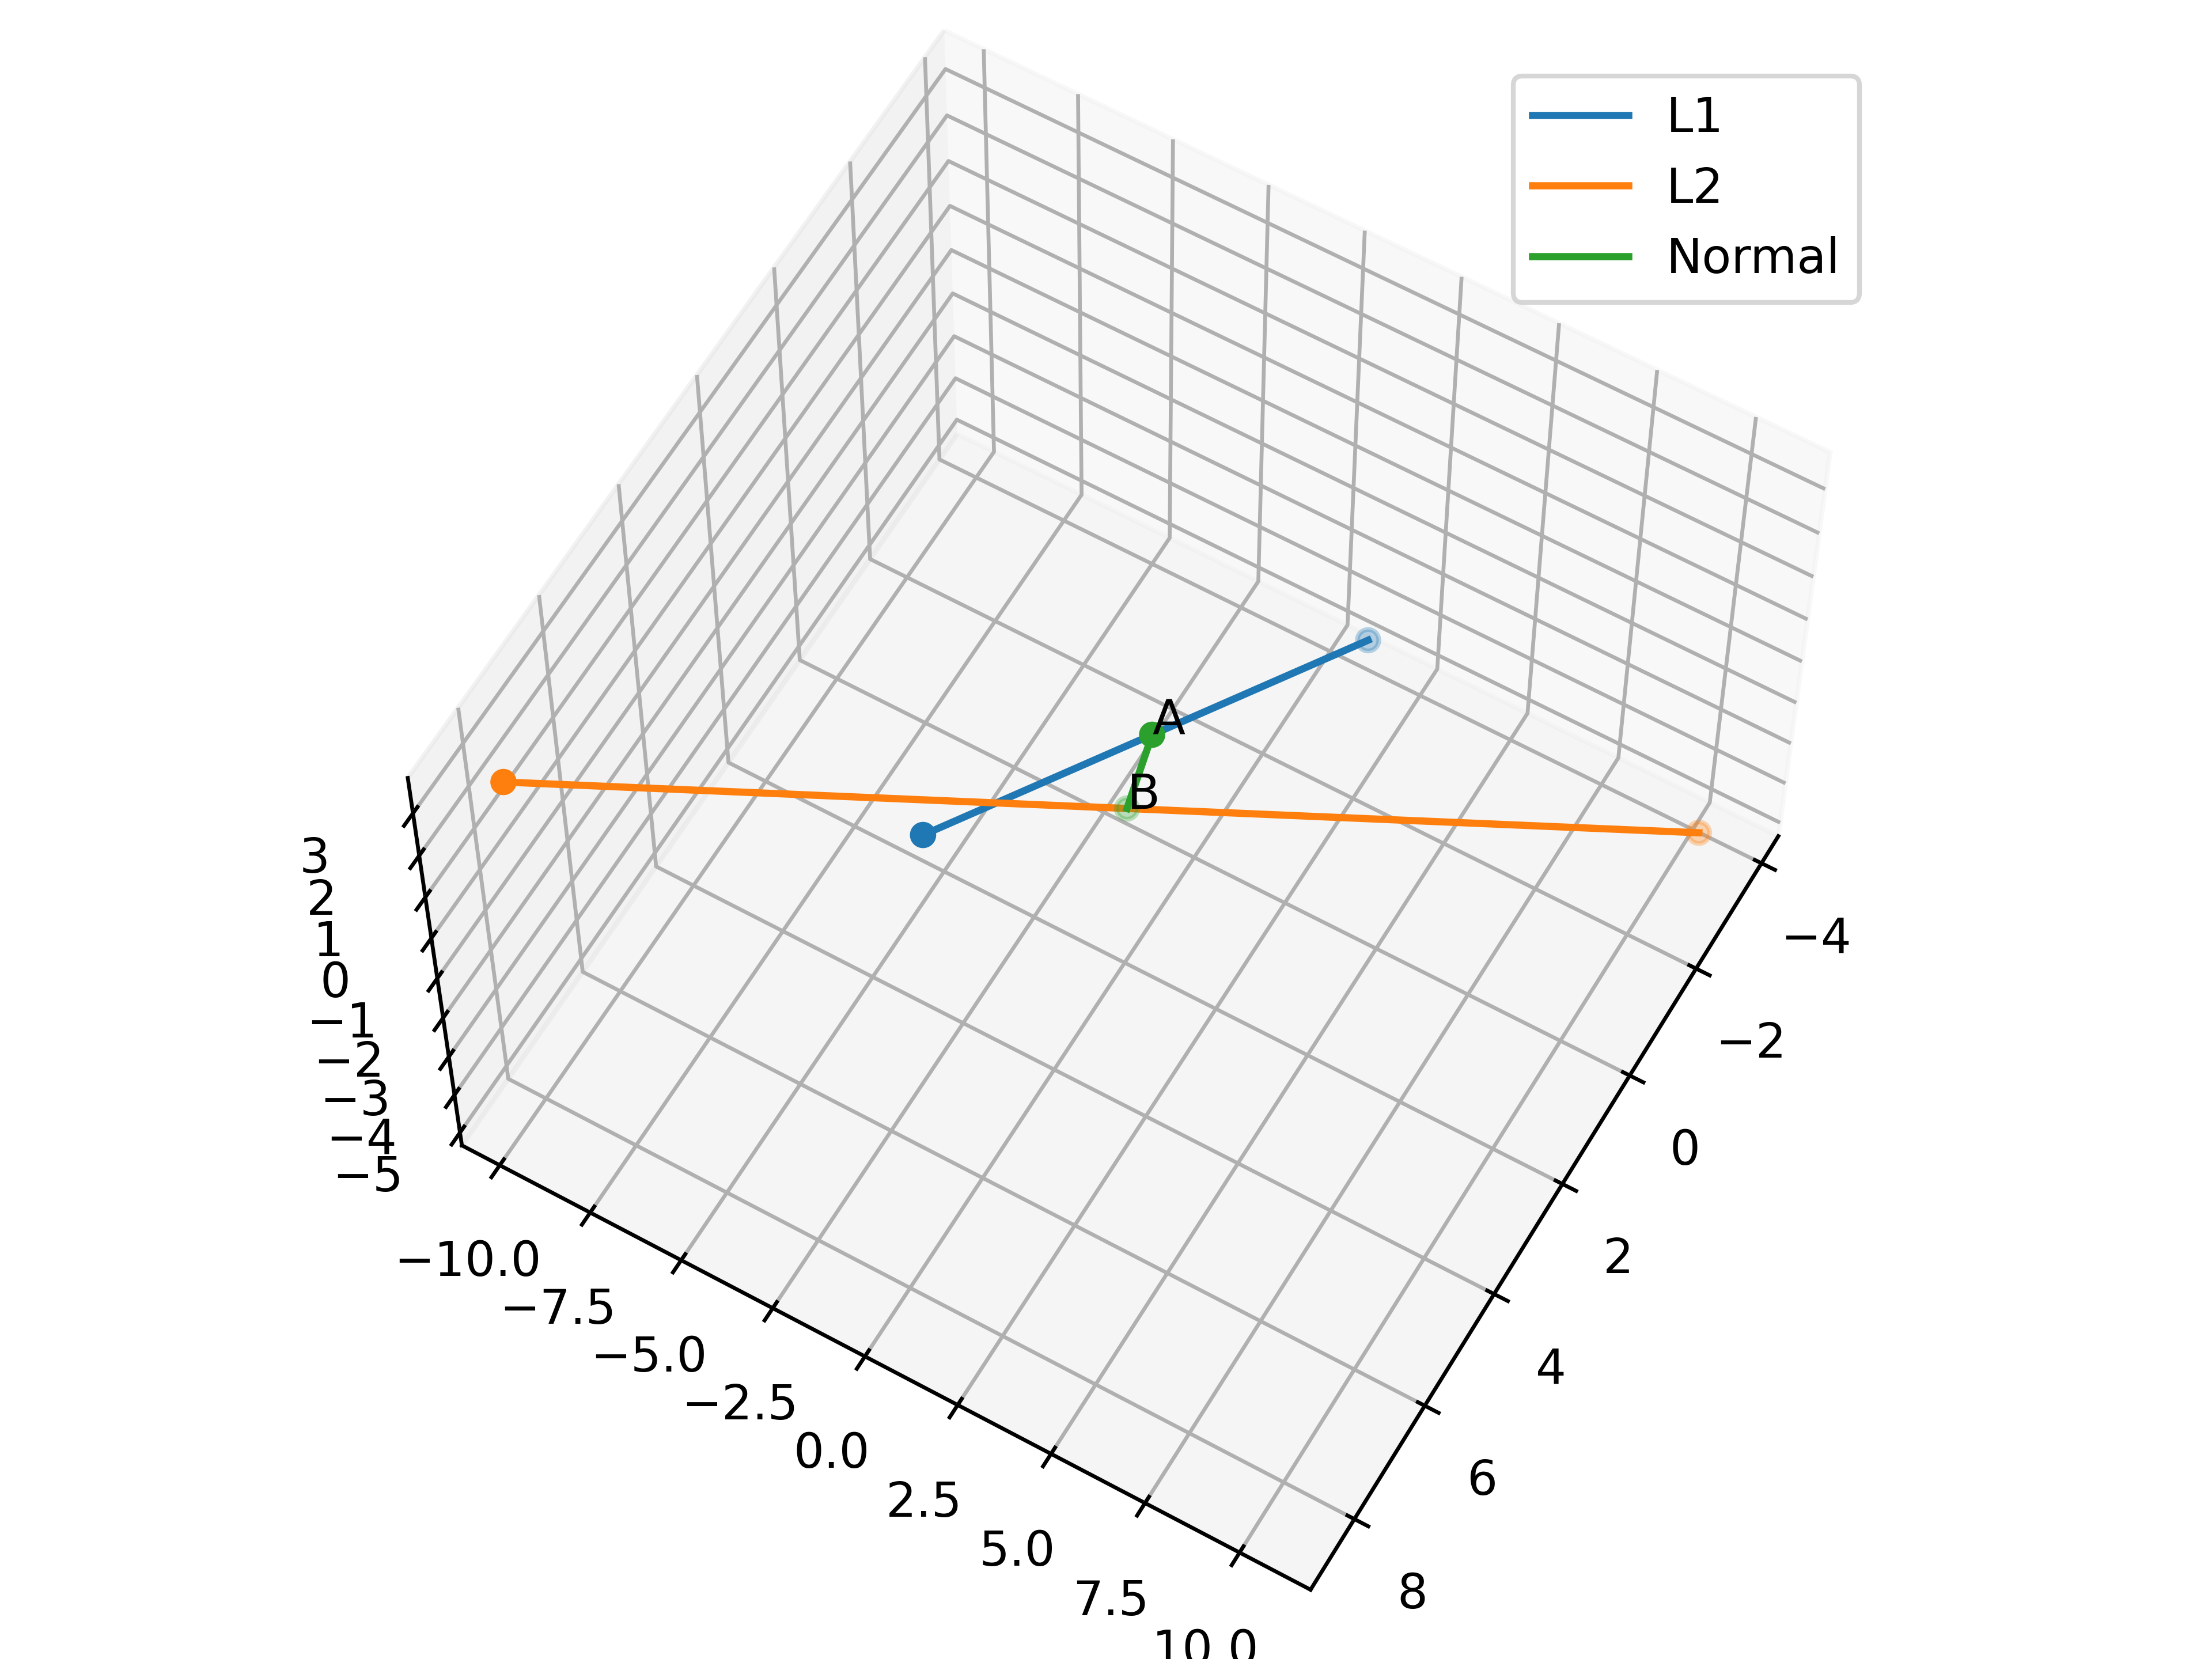
\includegraphics[width=\columnwidth]{chapters/12/11/2/e11/figs/skew.png}
\caption{}
	\label{fig:chapters/12/11/2/e11/}
\end{figure}
